% !TEX encoding = UTF-8
% !TEX TS-program = pdflatex
% !TEX root = ../tesi.tex

%**************************************************************
\chapter{Algoritmo per il calcolo della traiettoria}
\label{cap:business-logic}
%**************************************************************

\intro{In questa sezione si documenterà la realizzazione della business logic per il calcolo della traiettoria e l'interfacciamento con il drone.}\\

%**************************************************************

\section{Strumenti utilizzati}
Il linguaggio scelto per sviluppare questa componente della Proof of Concept è Java nella versione 11. Si è usato l'IDE IntelliJ IDEA Education, il quale offre un ambiente di sviluppo integrato sia per Java che per Python. In questo modo è stato possibile eseguire il server per le predizioni insieme al modulo del programma in Java che si interfaccia con questo in modo molto semplificato.

\section{Architettura generale}
L'architettura data all'applicazione è quella del monolite a strati, di cui si può vedere una rappresentazione ad alto livello nella figura \ref{fig:layered_architecture}. Il principale vantaggio che si ottiene dall'adozione di questa architettura è alta testabilità: infatti è molto semplice creare delle componenti di mock o addirittura layer interi che sostituiscono quelli reali, al fine di testare gli strati superiori.
    
\begin{figure}
    \centering
    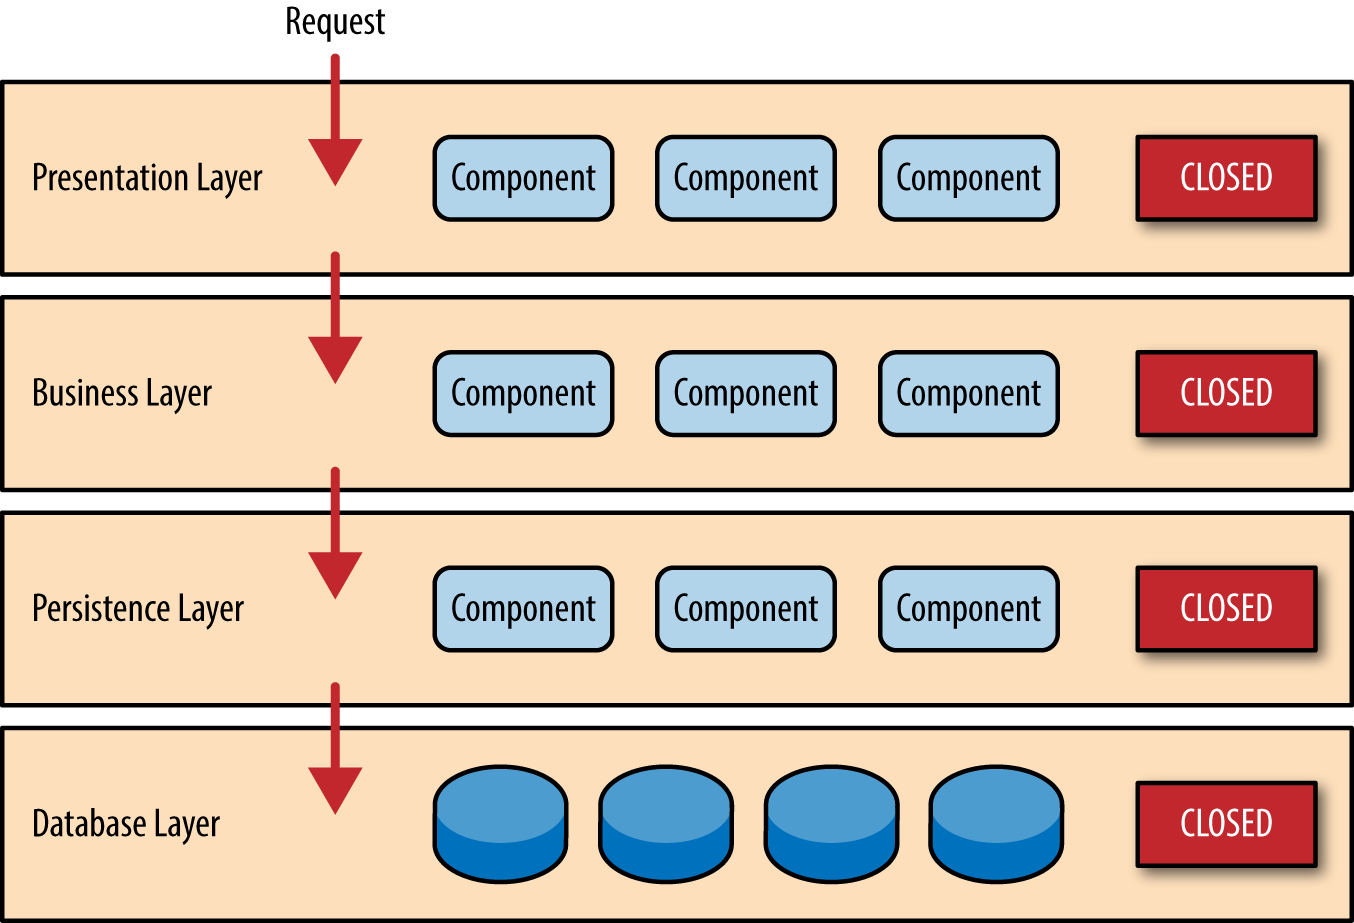
\includegraphics[width=\textwidth]{immagini/layered_archiecture.png}
    \caption{Architettura monolitica a strati}
    \label{fig:layered_architecture}
\end{figure}

\subsection{Strato di persistenza}

\subsubsection{Persistenza dei dati}
È stata prevista la possibilità per lo strato superiore di salvare il suo stato in un file oppure in un database. In particolare è utile per salvare i dati raccolti dal drone durante le rilevazioni e non dover ricalcolare tutto il percorso da zero ad ogni avvio. Si può vedere la struttura delle classi in figura \ref{fig:class_diagram_persistence}.

\begin{figure}
    \centering
    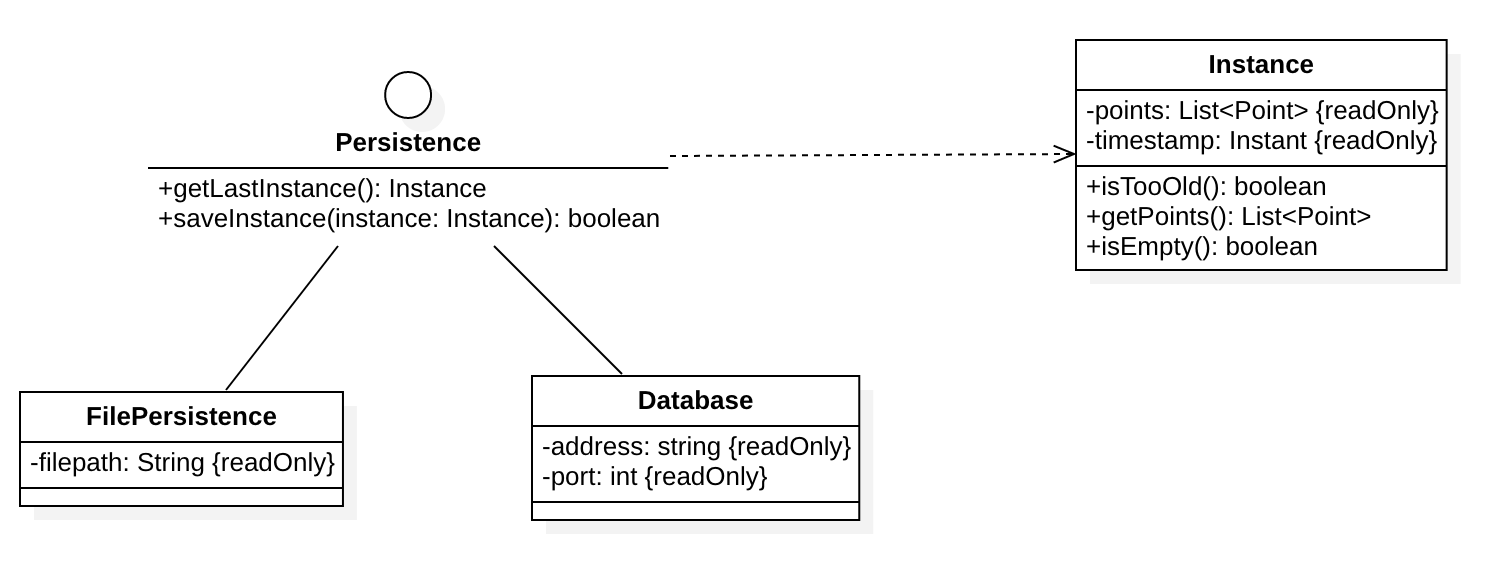
\includegraphics[width=\textwidth]{immagini/persistence_classes.png}
    \caption{Diagramma delle classi per la persistenza dei dati}
    \label{fig:class_diagram_persistence}
\end{figure}

\subsubsection{Interfacciamento con la rete neurale}
A questo livello, oltre alle classi per la persistenza che si interfacciano con il database e i file, c'è il server che espone la rete neurale per le predizioni. Di conseguenza lo strato di persistenza comprende l'insieme di quelle classi addette a comporre la richiesta HTTP da inviare all'end-point, le quali sono collocate nel package prediction. In particolare all'interno di questo troviamo la classe NeuralNetworkClient che contiene tra i suoi campi dati un oggetto con il tipo HttpClient, offerta dalla libreria \verb|java.net|. Grazie a questo è possibile esporre nell'interfaccia pubblica della classe il metodo \verb|predict|, il quale prende come parametro una lista contenente i valori dello spettro luminoso (già interpolati in modo che siano uniformi con i valori con cui la rete è stata allenata) e ritorna un valore interno $k \in \{0 .. 6 \}$ che indica la classe di appartenenza tra quelle elencate nel capitolo \ref{cap:machine-learning}. Questo metodo ha inoltre il compito di gestire eventuali eccezioni lanciate durante la chiamata al server, ritornando un valore negativo.\\
È possibile vedere il diagramma delle classi per questa parte di layer nella figura \ref{fig:class_diagram_neural_network}.

\begin{figure}
    \centering
    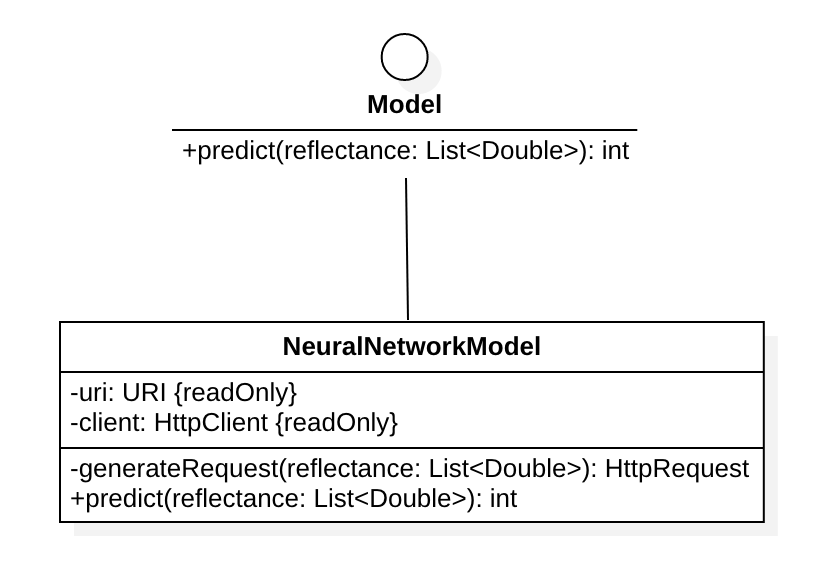
\includegraphics[width=0.8\textwidth]{immagini/model_classes.png}
    \caption{Diagramma delle classi per l'interfacciamento con la rete neurale}
    \label{fig:class_diagram_neural_network}
\end{figure}

\subsection{Strato di business}
Salendo, a questo livello, troviamo l'insieme delle classi atte al calcolo del percorso che il drone dovrà eseguire. Si riporta nell'algoritmo \ref{alg:calculate_track} lo pseudo-codice per il calcolo del percorso. L'input sono due array paralleli $x$ e $y$ di grandezza $n$ (con $n$ il numero di punti da attraversare) contenenti le coordinate. Possiamo notare come questo problema è riconducibile ad un grafo completo $K_n$, in cui ogni nodo è connesso da un arco a tutti gli altri. Ognuno di questi archi ha un costo di percorrenza che dipende direttamente dalla distanza tra i due punti, espressi in coordinate. Ci troviamo di fronte al problema del commesso viaggiatore.\\
È possibile vedere il diagramma delle classi per questo layer nella figura \ref{fig:class_diagram_business}.

\begin{figure}
    \centering
    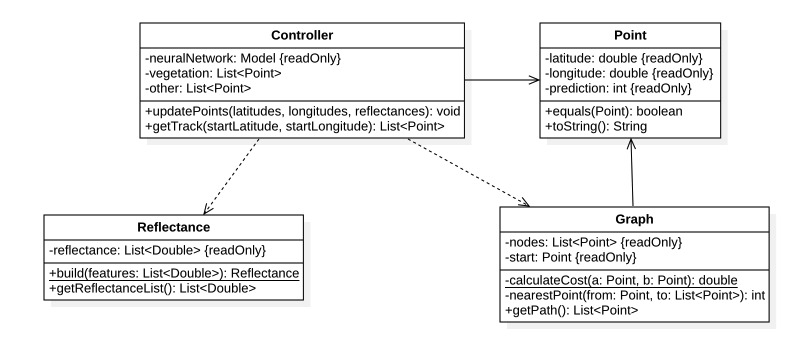
\includegraphics[width=\textwidth]{immagini/business_classes.png}
    \caption{Diagramma delle classi per lo strato di business}
    \label{fig:class_diagram_business}
\end{figure}

\subsubsection{Problema del commesso viaggiatore}
Il nome nasce da una tipica rappresentazione del problema: dato un insieme di città da visitare una ed una sola volta e note le distanze tra queste, trovare il tragitto di minima percorrenza che un commesso viaggiatore deve eseguire per effettuare tutte le consegne e ritornare al punto di partenza. È stato dimostrato che questo problema è \textit{NP-hard}, in quanto non esiste un algoritmo che lo risolva in tempo polinomiale. L'unico metodo di risoluzione efficace è l'enumerazione totale dei possibili percorsi, che ricade nella classe di complessità computazionale $\theta(n!)$.

\subsubsection{Algoritmo euristico di risoluzione}
Per affrontare il problema si è deciso di realizzare un algoritmo euristico, ovvero la cui soluzione prodotta è probabilmente buona ma non ottima.
Come si può notare, il costo computazionale della procedura \verb|nearest_point| è lineare, dunque il costo totale della procedura rientra nella classe di algoritmi $\theta(n^2)$ con consumo di memoria costante. Considerando che nell'applicazione reale il valore di $n$ non raggiungerà mai valori elevati, il risultato è accettabile. Inoltre è possibile ottimizzare questo algoritmo durante l'implementazione rimuovendo i punti già inclusi nel cammino dagli array $x$ e $y$ invece di porre le coordinate a infinito.

\subsubsection{Dimostrazione di correttezza}
Assumendo la correttezza della funzione \verb|calculate_distance(x_a, y_a, x_b, y_b)| e che si completi in tempo $\theta(1)$ restituendo il valore della distanza tra i due punti identificati dalle coordinate passate come parametro, possiamo fornire una dimostrazione di correttezza dell'algoritmo. In particolare assumiamo che la PRE-condizione della funzione appena menzionata asserisca che i valori in ingresso identifichino le coordinate di due punti $A$ e $B$, i quali potrebbero coincidere; la POST-condizione invece stabilisce che venga ritornato un valore numerico, il quale identifica la distanza tra i due punti, dunque pari a $0$ se e solo se $A == B$.\\
Per dimostrare la correttezza della procedura riportata in \ref{alg:nearest_point}, è necessario dimostrare la correttezza del ciclo al suo interno. In particolare l'invariante di ciclo è che all'inizio di ogni iterazione la variabile $minIndex$ contiene l'indice del punto più vicino dal punto con coordinate $x\_from$ e $y\_from$ contenuto nei sotto array $x\_to[1 \dotso i-1]$ e $y\_to[1 \dotso i-1]$, mentre la variabile $minDistance$ contiene il valore della distanza tra il punto di partenza e il punto contenuto nell'array nella cella $minIndex$.

\begin{itemize}
    \item Inizializzazione: prima dell'inizio del ciclo i sottoarray $x\_to[1 \dotso i-1]$ e $y\_to[1 \dotso i-1]$ sono vuoti, dunque non esiste un punto che abbia una distanza valida dal punto di partenza.
    \item Conservazione: assumendo che prima di ogni iterazione l'invariante sia rispettato, possiamo notare che aggiungendo l'elemento i-esimo ai sottoarray finora considerati l'invariante resta valido, infatti il punto più vicino viene aggiornato solo se la sua distanza è minore di quella più piccola finora individuata.
    \item Conclusione: dopo l'ultima iterazione, quando $i == n$ sappiamo che $minIndex$ contiene l'indice del punto più vicino a quello di partenza compreso in $x\_to[1 \dotso n]$ e $x\_to[1 \dotso n]$, dunque non resta che ritornare tale valore.
\end{itemize}

Una volta fatta questa dimostrazione è banale dedurre la correttezza dell'algoritmo di calcolo del percorso riportato in \ref{alg:calculate_track}. La PRE-condizione di questo è che i punti negli array $x[1 \dotso n]$ e $y[1 \dotso n]$ non siano duplicati e che il punto di partenza identificato dalle coordinate $x\_start$ e $y\_start$ non sia un valore contenuto negli array. La POST-condizione è che gli array $x\_path[1 \dotso n+1]$ e $y\_path[1 \dotso n+1]$ contengano esattamente i punti contenuti originariamente in $x$ e $y$ e alla posizione $n+1$ il punto di partenza, in modo che il percorso termini nello stesso punto da cui è partito. Inoltre i punti devono essere ordinati secondo una scelta greedy, ovvero ogni volta selezionando il più vicino dal punto precedente. L'invariante di ciclo asserisce quindi che $x\_prev$ e $y\_prev$ contengano l'ultimo punto aggiunto al percorso da cui valutare le distanze verso i possibili punti successivi e che i punti già inseriti nel cammino non vengano più considerati nel calcolo delle distanze.

\begin{itemize}
    \item Inizializzazione: prima dell'inizio del ciclo il punto precedente è quello di partenza, dunque l'invariante è verificato.
    \item Conservazione: assumendo che l'invariante sia vero all'inizio dell'iterazione, dimostriamo il mantenimento della sua validità. Viene invocata la funzione \verb|nearest_point(x_from, y_from, x_to, y_to)| passando come valori per $x\_from$ e $y\_from$ il punto precedente, mentre come valori $x\_to$ e $y\_to$ gli array contenenti le coordinate con le possibili destinazioni. Avendo precedentemente dimostrato la correttezza di questa funzione, sappiamo che ritorna l'indice intero $next \in \{ 1, \dotso, n \}$ che identifica il punto più vicino a quello precedente contenuto negli array $x$ e $y$. Aggiungiamo quindi questo punto al cammino in posizione i-esima, ovvero subito dopo il precedente. Inoltre viene posto il valore di questo punto a infinito, in modo che nel calcolo del punto più vicino nelle future iterazioni questo non venga mai considerato. Aggiorniamo quindi i valori delle coordinate $x\_prev$ e $y\_prev$ con quelle del punto appena incluso nel cammino, che sarà il punto precedente per la prossima iterazione.
    \item Conclusione: al termine del ciclo i sottoarray $x\_path[1\dotso n]$ e $y\_path[1 \dotso n]$ contengono i punti ordinati secondo la scelta greedy prima menzionata, non resta quindi che aggiungere in posizione ($n+1$)-esima il punto di partenza in modo che il cammino termini dov'è cominciato.
\end{itemize}

\begin{algorithm}
    \caption{Algoritmo per il calcolo del percorso}
    \label{alg:calculate_track}
    \begin{algorithmic}
        \Require array $x[1 \dotso n]$ e $y[1 \dotso n]$ senza valori duplicati
        \Require $x\_start \notin x$ e $y\_start \notin y$
        \Ensure $x\_path[1 \dotso n+1]$ e $y\_path[1 \dotso n+1]$
        \State Inizializza array $x\_path[1 \dotso n+1]$, $y\_path[1 \dotso n+1]$
        \State $x\_prev \leftarrow x\_start$
        \State $y\_prev \leftarrow y\_start$
        \For{$i \leftarrow 1$ to $n$}
            \State $next \leftarrow \verb|nearest_point|(x\_prev,\  y\_prev,\  x,\  y)$
            \Comment Algoritmo \ref{alg:nearest_point}
            \State $x\_path[i] \leftarrow x[next]$
            \State $y\_path[i] \leftarrow y[next]$
            \State $x[next] \leftarrow \infty$
            \State $y[next] \leftarrow \infty$
            \State $x\_prev \leftarrow x\_path[i]$
            \State $y\_prev \leftarrow y\_path[i]$
        \EndFor
        \State $x\_path[n+1] \leftarrow x\_start$
        \State $y\_path[n+1] \leftarrow y\_start$
        \State \Return $(x\_path , y\_path)$
    \end{algorithmic}
\end{algorithm}

\begin{algorithm}
    \caption{Procedura nearest point}
    \label{alg:nearest_point}
    \begin{algorithmic}
        \Require $x\_from$, $y\_from$ il punto di partenza
        \Require $x\_to[1 \dotso n]$, $y\_to[1 \dotso n]$ array con le $n$ destinazioni possibili differenti
        \Ensure $minIndex$ l'indice della posizione più vicina
        \State $minIndex \leftarrow -1$
        \State $minDistance \leftarrow \infty$
        \For{$i \leftarrow 1$ to $n$}
            \State $distance \leftarrow \verb|calculate_distance|(x\_from,\  y\_from,\  x\_to[i],\  y\_to[i])$
            \If{$distance < minDistance$}
                \State $minDistance \leftarrow distance$
                \State $minIndex \leftarrow i$
            \EndIf
        \EndFor
        \State \Return $minIndex$
    \end{algorithmic}
\end{algorithm}

\subsection{Strato di presentazione}
Questo livello ha il compito di esporre tutto il monolite all'esterno.
Va premesso che il drone che andrà ad interfacciarsi con questo software avrà una scheda Arduino, dunque in grado di effettuare chiamate HTTP ad un end-point indicato grazie al linguaggio C++.
Nel nostro specifico caso si tratta di esporne tre:
\begin{itemize}
    \item \verb|/track|: questo risponde a chiamate HTTP di tipo GET, viene invocato dal drone quando ha bisogno di conoscere il tracciato che deve percorrere;
    \item \verb|/data|: questo risponde a chiamate HTTP di tipo POST, viene invocato dal drone quando ha fatto delle rilevazioni con lo spettrometro e le invia al software in modo che il percorso di aggiorni. La risposta può essere un successo o un fallimento;
    \item \verb|/perimeter|: risponde a chiamate HTTP di tipo PATCH, serve a impostare il perimetro di sorvolo del drone.
\end{itemize}
È possibile vedere il diagramma delle classi per questo layer nella figura \ref{fig:class_diagram_presentation}. Le API sono state documentate seguendo lo standard OpenAPI 3.0.0.

\begin{figure}
    \centering
    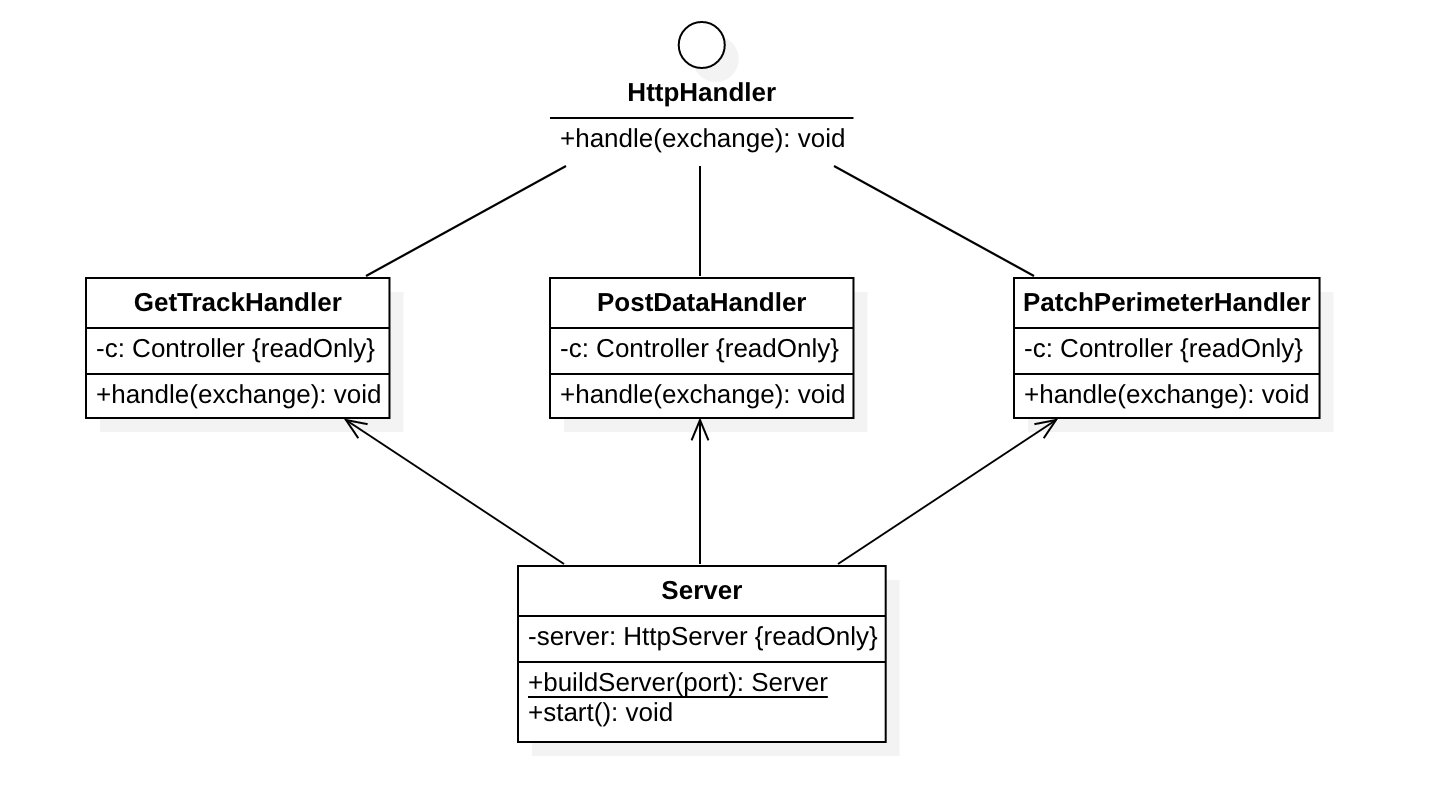
\includegraphics[width=0.8\textwidth]{immagini/presentation_classes.png}
    \caption{Diagramma delle classi per lo strato di presentazione}
    \label{fig:class_diagram_presentation}
\end{figure}